\documentclass[10pt]{beamer}
\usepackage{amsmath}
\usepackage{mathtools}
%\documentclass[12pt]{beamerthemeSam.sty}
\usepackage{epsf}
\usefonttheme{professionalfonts} % using non standard fonts for beamer
\usefonttheme{serif} % default family is serif


%\usepackage{pstricks}
%\usepackage[orientation=portrait,size=A4]{beamerposter}
\geometry{paperwidth=160mm,paperheight=120mm}
%DT favorite definitions
\def\LL{\left\langle}	% left angle bracket
\def\RR{\right\rangle}	% right angle bracket
\def\LP{\left(}		% left parenthesis
\def\RP{\right)}	% right parenthesis
\def\LB{\left\{}	% left curly bracket
\def\RB{\right\}}	% right curly bracket
\def\PAR#1#2{ {{\partial #1}\over{\partial #2}} }
\def\PARTWO#1#2{ {{\partial^2 #1}\over{\partial #2}^2} }
\def\PARTWOMIX#1#2#3{ {{\partial^2 #1}\over{\partial #2 \partial #3}} }

\def\rightpartial{{\overrightarrow\partial}}
\def\leftpartial{{\overleftarrow\partial}}
\def\diffpartial{\buildrel\leftrightarrow\over\partial}

\def\BC{\begin{center}}
\def\EC{\end{center}}
\def\BI{\begin{itemize}}
\def\EI{\end{itemize}}
\def\BE{\begin{displaymath}}
\def\EE{\end{displaymath}}
\def\BEA{\begin{eqnarray*}}
\def\EEA{\end{eqnarray*}}
\def\BNEA{\begin{eqnarray}}
\def\ENEA{\end{eqnarray}}
\def\EL{\nonumber\\}


\newcommand{\map}[1]{\frame{\frametitle{\textbf{Course map}}
\centerline{\includegraphics[height=0.86\paperheight]{../../map/#1.png}}}}
\newcommand{\wmap}[1]{\frame{\frametitle{\textbf{Course map}}
\centerline{\includegraphics[width=0.96\paperwidth]{../../map/#1.png}}}}

\newcommand{\etal}{{\it et al.}}
\newcommand{\gbeta}{6/g^2}
\newcommand{\la}[1]{\label{#1}}
\newcommand{\ie}{{\em i.e.\ }}
\newcommand{\eg}{{\em e.\,g.\ }}
\newcommand{\cf}{cf.\ }
\newcommand{\etc}{etc.\ }
\newcommand{\atantwo}{{\rm atan2}}
\newcommand{\Tr}{{\rm Tr}}
\newcommand{\dt}{\Delta t}
\newcommand{\op}{{\cal O}}
\newcommand{\msbar}{{\overline{\rm MS}}}
\def\chpt{\raise0.4ex\hbox{$\chi$}PT}
\def\schpt{S\raise0.4ex\hbox{$\chi$}PT}
\def\MeV{{\rm Me\!V}}
\def\GeV{{\rm Ge\!V}}

%AB: my color definitions
%\definecolor{mygarnet}{rgb}{0.445,0.184,0.215}
%\definecolor{mygold}{rgb}{0.848,0.848,0.098}
%\definecolor{myg2g}{rgb}{0.647,0.316,0.157}
\definecolor{abtitlecolor}{rgb}{0.0,0.255,0.494}
\definecolor{absecondarycolor}{rgb}{0.0,0.416,0.804}
\definecolor{abprimarycolor}{rgb}{1.0,0.686,0.0}
\definecolor{Red}           {cmyk}{0,1,1,0}
\definecolor{Grey}           {cmyk}{.7,.7,.7,0}
\definecolor{Blue}          {cmyk}{1,1,0,0}
\definecolor{Green}         {cmyk}{1,0,1,0}
\definecolor{Brown}         {cmyk}{0,0.81,1,0.60}
\definecolor{Black}         {cmyk}{0,0,0,1}
\definecolor{A}{rgb}{0.8,0.0,0.0}
\definecolor{B}{rgb}{0.0,0.6,0.0}
\definecolor{C}{rgb}{0.4,0.4,0.0}
\definecolor{D}{rgb}{0.0,0.0,0.5}
\definecolor{E}{rgb}{0.4,0.4,0.4}
\usetheme{Madrid}


%AB: redefinition of beamer colors
%\setbeamercolor{palette tertiary}{fg=white,bg=mygarnet}
%\setbeamercolor{palette secondary}{fg=white,bg=myg2g}
%\setbeamercolor{palette primary}{fg=black,bg=mygold}
\setbeamercolor{title}{fg=abtitlecolor}
\setbeamercolor{frametitle}{fg=abtitlecolor}
\setbeamercolor{palette tertiary}{fg=white,bg=abtitlecolor}
\setbeamercolor{palette secondary}{fg=white,bg=absecondarycolor}
\setbeamercolor{palette primary}{fg=black,bg=abprimarycolor}
\setbeamercolor{structure}{fg=abtitlecolor}

\setbeamerfont{section in toc}{series=\bfseries}

%AB: remove navigation icons
\beamertemplatenavigationsymbolsempty
\title[Problem solving: kinematics]{
  \textbf {Problem solving: kinematics (II)}\\
%\centerline{}
%\centering
%\vspace{-0.0in}
%\includegraphics[width=0.3\textwidth]{propvalues_0093.pdf}
%\vspace{-0.3in}\\
%\label{intrograph}
}

<<<<<<< HEAD
\author[W. Freeman] {Physics 211\\Syracuse University, Physics 211 Spring 2022\\Walter Freeman}
=======
\author[W. Freeman] {Physics 211\\Syracuse University, Physics 211 Spring 2023\\Walter Freeman}
>>>>>>> 8c055e0 (asdf)

\date{\today}

\begin{document}

\frame{\titlepage}

\frame{\frametitle{\textbf{Announcements}}
\large
\BI
<<<<<<< HEAD
\item{Homework 2 due date is {\bf this Friday}}
=======
\item{Homework 2 due date is {\bf this Thursday or Friday}}
>>>>>>> 8c055e0 (asdf)
\item{Exam 1 is next Tuesday}
  \BI
\item{No homework due next week}
\item{HW2 problems are similar to those on Exam 1}
<<<<<<< HEAD
\item{Recitation Friday is your group practice exam}
\item{If you must miss Friday, notify your TA in advance}
=======
\item{Recitation Thursday/Friday is your group practice exam}
\item{If you must miss the group exam, notify your TA and your group in advance}
>>>>>>> 8c055e0 (asdf)
\BI
\item{Weekend: Exam review in the auditorium, Saturday, 5PM-8PM.}
  \EI
\EI
\EI
}

<<<<<<< HEAD
\frame{
	\begin{center}
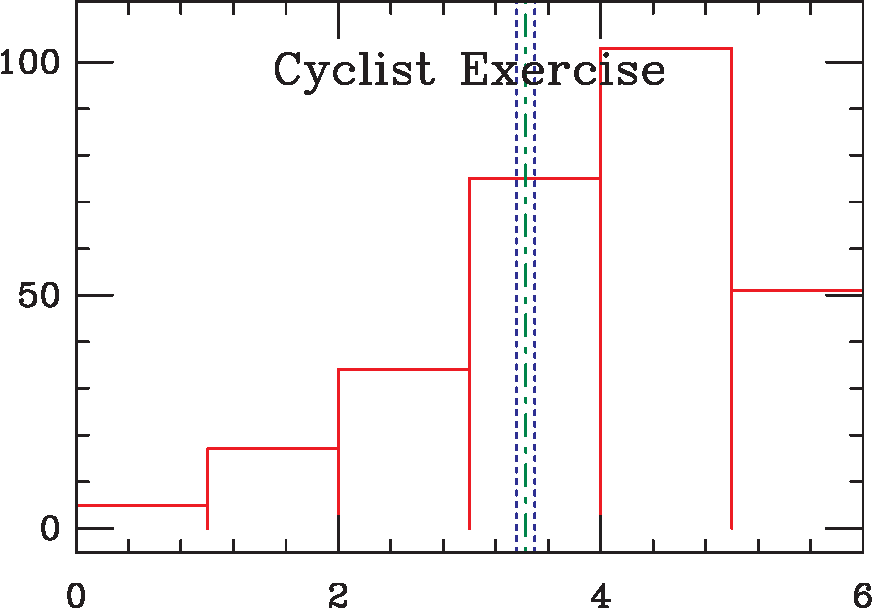
\includegraphics[width=0.4\textwidth]{cyclist-histogram.pdf}\hspace{0.1\textwidth}	
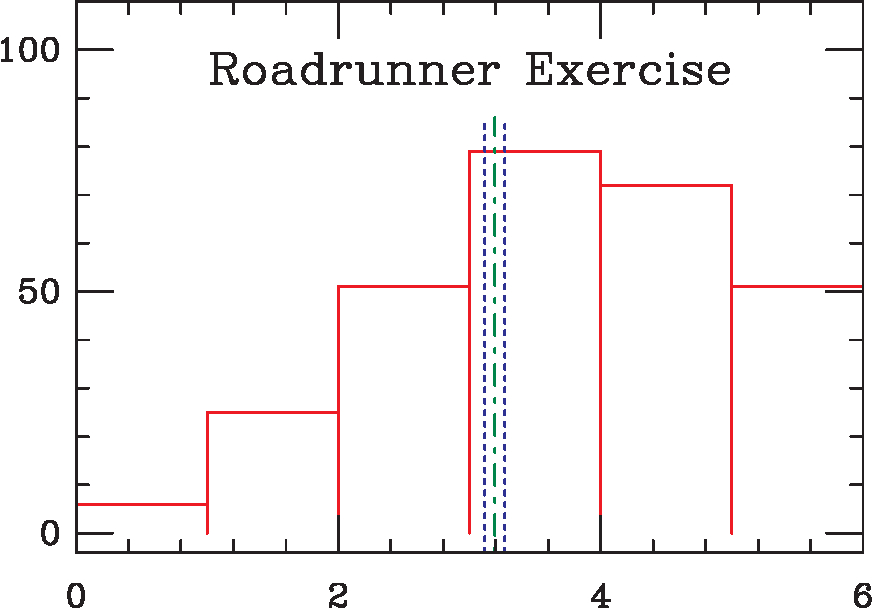
\includegraphics[width=0.4\textwidth]{roadrunner-histogram.pdf}\vspace{0.05\textwidth}
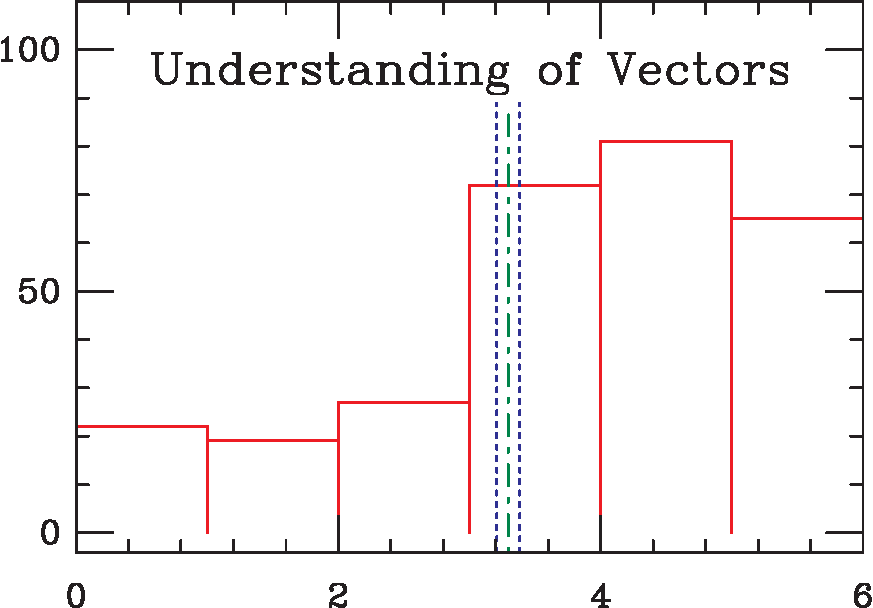
\includegraphics[width=0.4\textwidth]{vectors-histogram.pdf}\hspace{0.1\textwidth}
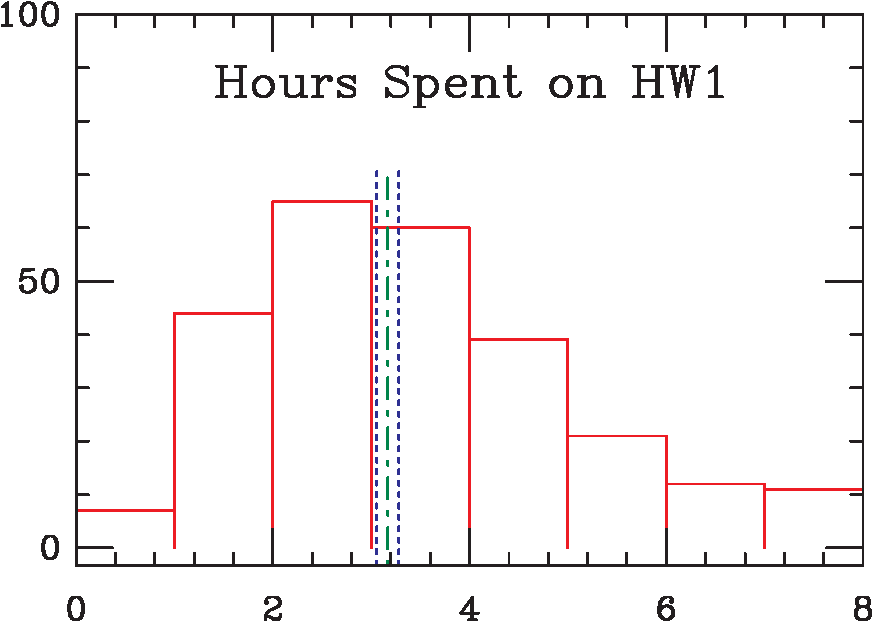
\includegraphics[width=0.4\textwidth]{hw1-histo.pdf}
\end{center}
	
}

\frame{\frametitle{\textbf{Makeup / study opportunities}}
	We've arranged the following series of catchup/makeup/study sessions this week. All sessions will meet in the Clinic but may move to another room if need be.
	
	\begin{itemize}\color{A}
		\item Tuesday 9:45-10:30 -- I'll be in the Clinic helping with whatever people need.
		\item Tuesday 2:00-3:45 -- I'll be in the Clinic.
		\item Tuesday 5-6:30 -- Mac and Kiersten:
		\begin{itemize}
			\color{A}
			\item General mathematics review
			\item Review of vectors (for those who missed Friday's recitation)
		\end{itemize}\pause\color{C}
	     \item Wednesday 3:00-4:30: Adil and Kiersten:
	     \begin{itemize}
	     	\color{C}
	     	\item Catchup if you missed class due to COVID (focusing on beginning of semester)
	     	\item Homework help
	     \end{itemize}
     \item Wednesday 4:30-5:30: I'll be in the Clinic.
     \item Wednesday 5:30-7:00: Adil -- Catchup if you missed a week from COVID (focusing on week 2)\pause
     \color{B}
     \item Thursday 9:45-10:30 -- I'll be in the Clinic helping with whatever people need.
     \item Thursday 3:00-5:00: Adam P, Chris.
     \begin{itemize}
     	\color{B}
     	\item ``How to Set Up Problems''
     	\item Homework help
     \end{itemize}
 \item Thursday 5:00-6:00 -- I'll be in the Clinic (maybe)
 \item Thursday 6:00-8:30 -- AJ: ``Bring Your Questions'' -- review of homework and recitation exercises by request\pause\color{D}
 \item Friday all day: Group Exam Review. Not sure how something in the group exam worked? Come by to discuss!
	\end{itemize}
}
=======


\frame{\frametitle{\textbf{Help hours this week}}
	
	
	Homework help / general assistance:
	\begin{itemize}\color{A}
		\item Anytime in the Physics Clinic (there is usually a tutor there)
		\item Tuesday 2:00-4:00 (Walter)
		\item Wednesday 3:00-5:00 (Walter)
		\item Thursday 3:00-5:00 (Walter)
	\end{itemize}
  \bigskip\bigskip
\color{C}
Wednesday night: Extra assistance session in room B129E (probably 6:30-8:30pm -- I'll announce by email this afternoon). Topics:


\BI
\color{C}
\item ``Setting up problems''
\item Algebra review
\item Trigonometry review
\item The quadratic formula
\item Vectors (if you missed Thurs/Fri recitation last week)
\item Position/velocity/acceleration graphs
\EI

\bigskip\bigskip
\color{B}
  Friday all day: Group Exam Review. Not sure how something in the group exam worked? Come by to discuss!  
  
\color{D}
  \bigskip\bigskip

Saturday, 5:00-8:00: Exam 1 Review (Stolkin Auditorium)
  

}

>>>>>>> 8c055e0 (asdf)



\frame{\frametitle{\textbf{Exam 1}}
 \BI
 \item{The exam covers kinematics in one and two dimensions}
 \item{Kinematics: how are an object's position, velocity, and acceleration related?}
   \pause
 \item{\color{Red}The exam will be somewhat easier than the homework.}
<<<<<<< HEAD
   \pause
 \item{You may use any ordinary calculator or graphing calculator on the exam, but no cellphones or computers, or Ti N-spire CAS level devices}
 \item{Students who do not speak English well: I will try to use only simple English on the exam, but if you like you may bring a dictionary}
 \item{Bring: your calculator, pencils, and your physics smarts (one-eyed kitten optional)}
   \pause
\item{Review session in class on Thursday}
=======
 \bigskip
   \pause
 \item{You may use any ordinary calculator or graphing calculator on the exam, but no cellphones or computers, or Ti N-spire CAS level devices}
 \item{Students who do not speak English well: I will try to use only simple English on the exam, but if you like you may bring a dictionary}
 \bigskip
 \item{Bring: your calculator, pencils, your physics smarts, and kitten/dog treats}
   \pause
\bigskip
>>>>>>> 8c055e0 (asdf)
\item{You are allowed to bring one side of one page of notes that {\it you handwrite yourself} on Tuesday}
\item You do not {\it need} to bring notes; I will give you the kinematics relations on a reference page
\BI
\item No typed notes unless you have a disability that prevents you from writing
\item Your friend can't write it
\item You can't print stuff from the internet
\pause
\item It won't help you as much anyway 
  \EI
\EI
}

\frame{\frametitle{\textbf{Exam 1, promises}}
  \BI
\item{There will be one problem where you need the quadratic formula}
  \BI
\item{... this means interpreting the two values it spits out}
  \EI
\item{There will be at least one instance where you need to interpret or sketch position, velocity, and acceleration graphs}
<<<<<<< HEAD
\item{You will {\it not} need to compute derivatives or integrals algebraically}
\item{The exam will be four problems, plus possibly a few short-answer questions}
=======
\item There will be at least one problem with ``piecewise constant'' acceleration (bicycle problem on HW1, rocket problem in Week 2 Recitation 1)
\item{You will {\it not} need to compute derivatives or integrals algebraically}
\item{The exam will be four problems}
>>>>>>> 8c055e0 (asdf)
  \EI
}

\frame{\frametitle{\textbf{Last time}}
  \Large
  \BI
  \item{Vectors: objects with direction and magnitude.}
  \BI
  \item{Two representations:}
  \large
  \pause
  \item{Magnitude and direction (easiest to state, hardest to work with)}
  \item{Components (easiest to work with)}
  \item{Use trigonometry to go back and forth}
  \EI
  \item{One more piece of notation about vectors...}
  \EI
}
<<<<<<< HEAD

\frame{\frametitle{\textbf{Unit vectors}}
\large
In the ``ordered pair'' notation for vectors' components, you might write:

$$\vec v = (5,3)$$

But this is clunky, if you're trying to write it as part of an algebraic statement.

\bigskip

Instead we introduce ``unit vectors'', vectors with length 1, in the x, y, and z directions.

\begin{align*}
\hat i =& (1,0,0) \\
\hat j =& (0,1,0) \\
\hat k =& (0,0,1)
\end{align*}

\BI
\item{$\vec v = (5,3)$ : Ordered pair}
\item{$\vec v = 5 \hat i + 3 \hat j$ : Unit vectors}
\pause
\item{Both give you the same information, but unit vectors can be easier algebraically}
\item{They won't be essential for this class, but you should know the notation -- other people use it quite a bit, and I use it once on your homework}
\EI


}
=======
%
%\frame{\frametitle{\textbf{Unit vectors}}
%\large
%In the ``ordered pair'' notation for vectors' components, you might write:
%
%$$\vec v = (5,3)$$
%
%But this is clunky, if you're trying to write it as part of an algebraic statement.
%
%\bigskip
%
%Instead we introduce ``unit vectors'', vectors with length 1, in the x, y, and z directions.
%
%\begin{align*}
%\hat i =& (1,0,0) \\
%\hat j =& (0,1,0) \\
%\hat k =& (0,0,1)
%\end{align*}
%
%\BI
%\item{$\vec v = (5,3)$ : Ordered pair}
%\item{$\vec v = 5 \hat i + 3 \hat j$ : Unit vectors}
%\pause
%\item{Both give you the same information, but unit vectors can be easier algebraically}
%\item{They won't be essential for this class, but you should know the notation -- other people use it quite a bit, and I use it once on your homework}
%\EI
%
%
%}
>>>>>>> 8c055e0 (asdf)

\frame{

\Large

A word on positive and negative acceleration, velocity, ``speed'', and displacement:

\bigskip

When you choose your origin, you choose one direction to be positive, and the other to be negative. (Here: right = positive.)

\BI
\item An object with $x<0$ just means it's left of the origin.
\item An object with $v<0$ means it's moving to the left.
\item An object with $a<0$ means:
\BI
\item \color{A}A: it is moving to the left and gaining speed
\item \color{B}B: it is moving to the right and slowing down
\item \color{C}C: it is moving to the left and slowing down
\item \color{D}D: it is moving to the right and gaining speed
\EI
\EI
\pause
\bigskip
\BC
Do not confuse the sign of something with the sign of its derivative!
\EC
}

  

\frame{\frametitle{\textbf{Last time}}

    \large Acceleration, velocity, and position relationships are the same in 2D; they just apply {\color{Red}independently} for each component.
    \Large

    \begin{align*}
      \vec v(t) =&\, \vec at + \vec v_0 \\
      \vec s(t) =&\, \frac{1}{2}\vec a t^2 + \vec v_0 t + \vec s_0
    \end{align*}

    \pause

    \begin{align*}
      v_x(t) =& a_x t + v_{x,0} \\
      v_y(t) =& a_y t + v_{y,0} \\
    \end{align*}
    \pause
    \begin{align*}
      x(t) =&\,  \frac{1}{2}  a_x t^2 + v_{x,0} t + x_0\\
      \bigskip
      y(t) =&\, \frac{1}{2}  a_y t^2 + v_{y,0} t + y_0
    \end{align*}
  }
   \frame{\frametitle{\textbf{Working with variables}}
    \Large 
    \centerline{If you don't know the numerical value of a quantity yet, }
      \centerline{it's fine to leave it as a variable!}

    \bigskip

    \centerline{This is essential for solving many problems.}

    \pause

\bigskip
\bigskip

<<<<<<< HEAD
\centerline{Example from cannon problem:}
=======
\centerline{Example from the dog-and-ball problem:}
>>>>>>> 8c055e0 (asdf)

\begin{eqnarray*}
  x(t) = \frac{1}{2} a_x t^2 + {\color{Red}v_{x,0}} t + x_0 \\
  y(t) = \frac{1}{2} a_y t^2 + {\color{Red}v_{y,0}} t + y_0 
\end{eqnarray*}
}


   \frame{\frametitle{\textbf{Working with variables}}
    \Large 
  \centerline{If you don't know the numerical value of a quantity yet, }
      \centerline{it's fine to leave it as a variable!}

    \bigskip

    \centerline{This is essential for solving many problems.}



\bigskip
\bigskip

<<<<<<< HEAD
\centerline{Example from cannon problem:}
=======
\centerline{Example from dog-and-ball problem:}
>>>>>>> 8c055e0 (asdf)

\begin{align*}
  x(t) =& {\color{Red}v_{x,0}} t \\
    y(t) =& -\frac{1}{2} g t^2 + {\color{Red}v_{y,0}} t 
  \end{align*}


}




   \frame{\frametitle{\textbf{Working with variables}}
    \Large 
  \centerline{If you don't know the numerical value of a quantity yet, }
      \centerline{it's fine to leave it as a variable!}

    \bigskip

    \centerline{This is essential for solving many problems.}



\bigskip
\bigskip

<<<<<<< HEAD
\centerline{Example from cannon problem:}
=======
\centerline{Example from dog-and-ball problem:}
>>>>>>> 8c055e0 (asdf)

\begin{align*}
  x(t) =& {\color{Red}v_0 \cos 45^o} t \\
  y(t) =& -\frac{1}{2} g t^2 + {\color{Red}v_0 \sin 45^o} t \\
\end{align*}

  \centerline{(I leave the rest to you for now...)}

}



  \frame{\frametitle{\textbf{Problem solving: 2D kinematics, constant acceleration}}
    \large
    \begin{enumerate}
      \item 0. Draw a cartoon of the situation, and choose a coordinate system
      \item{1. If you have vectors in the ``angle and magnitude'' form ($\vec a, \vec v, \vec s$), convert them to components}
      \item{2. Write down the kinematics relations, separately for $x$ and $y$}
        \begin{itemize}
            \large
          \item{Many terms will usually be zero}
          \item{Freefall: $a_x = 0$, $a_y = -g$ (with conventional choice of axes)}
        \end{itemize}
      \item{3. Understand what instant in time you want to know about: ask the right question}
      \item{4. Put in what you know; solve for what you don't (using substitution, if necessary)}
      \item{5. Think about the physical meaning of your solution}
    \end{enumerate}
  }

  \frame{\frametitle{\textbf{Problem solving: 2D kinematics, constant acceleration}}
    \large
    \begin{enumerate}
      \item 0. Draw a cartoon of the situation, and choose a coordinate system
      \item{1. If you have vectors in the ``angle and magnitude'' form ($\vec a, \vec v, \vec s$), convert them to components}
      \item{2. Write down the kinematics relations, separately for $x$ and $y$}
        \begin{itemize}
            \large
          \item{Many terms will usually be zero}
          \item{Freefall: $a_x = 0$, $a_y = -g$ (with conventional choice of axes)}
        \end{itemize}
      \item{\color{Red}3. Understand what instant in time you want to know about: ask the right question}
      \item{4. Put in what you know; solve for what you don't (using substitution, if necessary)}
      \item{5. Think about the physical meaning of your solution}
    \end{enumerate}
  }


<<<<<<< HEAD

=======
 \frame{


\huge \begin{center} Homework questions? \end{center}

}
>>>>>>> 8c055e0 (asdf)
  \frame{\frametitle{\textbf{``What instant in time do you know about?''}}
  \large
{  \color{Red}This is often the most difficult part of problems: it requires thought, not just math.}

  \bigskip
  \bigskip
  \bigskip


\Large
You throw a ball upward over a hole of height $h$. Your position is the origin, and up is positive.

\bigskip

What condition means ``the ball has hit the ground''?

\BI
\item{\color{A}A: $y=0$}
\item{\color{B}B: $y=h$}
\item{\color{C}C: $y=-h$}
\item{\color{D}D: $v_y=0$}
\EI
}



  \frame{\frametitle{\textbf{``What instant in time do you know about?''}}


\Large
You throw a ball upward off of a cliff of height $h$. The top of the cliff is the origin, and up is positive.

\bigskip
\bigskip
\bigskip

What condition means ``the ball is at its highest point?''?

\BI
\item{A: $y=0$}
\item{B: $v_y=0$}
\item{C: $y=h$}
\item{D: $y$ is a maximum}
\EI
}


\frame{\frametitle{\textbf{A football player}}
\Large
A football player kicks the ball at 15 $m/s$ at an angle of 30 degrees above the horizontal.

\bigskip
\bigskip

How can we frame the question ``How far does the ball go?'' in terms of our variables?

\bigskip

\BI
\Large
\item{A: What is $x$ at the same time that $v_x$ is zero?}
\item{B: What is $y$ at the same time that $x$ is is zero?}
\item{C: What is $x$ at the same time that $y$ is zero?}
\item{D: What is $x$ at the same time that $v_y$ is zero?}
\EI
}

\frame{\frametitle{\textbf{A football player}}
\large
\BI
\item{A football player kicks the ball at 15 $m/s$ at an angle of 30 degrees above the horizontal.}
\item{If the field is level ground, how far does the ball go?}
  \pause
\item{How high does the ball go?}
  \pause
\item{How fast is it traveling at its highest point?}
  \pause
\item{How fast is it traveling when it strikes the ground?}
  \EI
}




\frame{\frametitle{\textbf{A football player}}
\large
\BI
\item{A football player kicks the ball at 15 $m/s$ at an angle of 30 degrees above the horizontal.}
\item{If the field is level ground, how far does the ball go?}
\item{How high does the ball go?}
\item{How fast is it traveling at its highest point?}
\item{How fast is it traveling when it strikes the ground?}
\EI

\bigskip

What is $v_{0,x}$?

\bigskip

\color{A}A: $v_0 \cos \theta$ \\
\color{B}B: $v_0 \sin \theta$ \\
\color{C}C: $v_0 \tan \theta$ \\
\color{D}D: $v_0$ \\
}


\frame{\frametitle{\textbf{A football player}}
	\large
	\BI
	\item{A football player kicks the ball at 15 $m/s$ at an angle of 30 degrees above the horizontal.}
	\item{If the field is level ground, how far does the ball go?}
	\item{How high does the ball go?}
	\item{How fast is it traveling at its highest point?}
	\item{How fast is it traveling when it strikes the ground?}
	\EI
	
	\bigskip
	
	What is $v_{0,y}$?
	
	\bigskip
	
	\color{A}A: $v_0 \cos \theta$ \\
	\color{B}B: $v_0 \sin \theta$ \\
	\color{C}C: $v_0 \tan \theta$ \\
	\color{D}D: $v_0$ \\
}

\frame{\frametitle{\textbf{A football player}}
\large
\BI
\item What changes if I put the football player up on a cliff?
\pause
\item What changes if they are kicking the ball up to someone on a cliff?
\pause
\item What changes if I want to know what velocity they need to kick the ball to midfield? 
\pause
\item What changes if I have air resistance?
\EI
}


\frame{\frametitle{\textbf{Throwing a rock off a cliff}}
\Large A hiker throws a rock horizontally off of a $h=100$ m tall cliff. If the rock strikes the ground $d=30$ m away, how hard did she 
  throw it? How fast was it going when it hit the ground? (Choose the origin at the base of the cliff, up/direction of throw as positive)}


\frame{

\Large

What is $v_{0,x}$ here?

\bigskip
\bigskip

\color{A}A: 0 \\
\color{B}B: 10/3 m/s\\
\color{C}C: You don't know {\it a priori} 
}


\frame{

\Large

What is $v_{0,y}$ here?

\bigskip
\bigskip

\color{A}A: 0 \\
\color{B}B: 9.8 m/s\\
\color{C}C: You don't know {\it a priori} 
}

\frame{

\Large

What is $a_{x}$ here?

\bigskip
\bigskip

\color{A}A: 0 \\
\color{B}B: -g\\
\color{C}C: +g\\
\color{D}D: You don't know {\it a priori} 
}

\frame{
\Large

What is $a_{y}$ here?

\bigskip
\bigskip

\color{A}A: 0 \\
\color{B}B: -g\\
\color{C}C: +g\\
\color{D}D: You don't know {\it a priori} 
}

\frame{
\Large

What is $x_0$ here?

\bigskip
\bigskip

\color{A}A: 0 \\
\color{B}B: h\\
\color{C}C: d\\
\color{D}D: You don't know {\it a priori} 
}

\frame{
\Large

What is $y_0$ here?

\bigskip
\bigskip

\color{A}A: 0 \\
\color{B}B: h\\
\color{C}C: d\\
\color{D}D: You don't know {\it a priori} 
}

\frame{
\Large
What question do you ask to find ``how hard did she throw it?''

\bigskip
\bigskip

\color{A}A: What value of $v_{x,0}$ makes it such that $x=d$ when $y=0$?\\
\color{B}B: What value of $v_{y,0}$ makes it such that $x=d$ when $y=h$?\\
\color{C}C: What is the value of $v_x$ when $y=0$? \\
\color{D}D: What is the magnitude of $\vec v$ when $y=0$?\\
\color{E}E: What is the magnitude of $\vec v_x$ when $y=h$?\\
} 

\frame{
\Large
What question do you ask to find ``how fast is it going when it hits the ground?''

\bigskip
\bigskip

\color{A}A: What is $v_x$ at the time when $v_y=0$?\\
\color{B}B: What is $v_x$ at the time when $y=0$?\\
\color{C}C: What is $v_y$ at the time when $y=h$?\\
\color{D}D: What is the magnitude of $\vec v$ when $y=0$?\\
\color{E}E: What is the magnitude of $\vec v$ when $y=h$?\\
} 

\frame{
\Large

What's the magnitude of $\vec v$?

\bigskip 
\bigskip 
\color{A}A: $v \cos \theta$\\
\color{B}B: $v \sin \theta$\\
\color{C}C: $\tan^{-1} \frac{v_x}{v_y}$\\ 
\color{D}A: $\sqrt{v_x^2 + v_y^2}$
}

\frame{\frametitle{\textbf{Throwing a stone onto a slope}}
  A hiker kicks a stone off of a mountain slope with an initial velocity of $v_0$ 3 m/s horizontally. If the mountain has a slope
  of 45 degrees, how far down the slope does it land? (Choose the origin as the starting point.)

\bigskip

\color{A}A: What is the magnitude of $\vec s$ when $x=y$?\\
\color{B}B: What is the magnitude of $\vec s$ when $x=-y$?\\
\color{C}C: What is the magnitude of $\vec s$ when $y=0$?\\
\color{D}D: What is y when $x=-y$?\\
\color{E}E: What is y when $x=0$?


\pause
\vspace{1in}

\begin{center}
	This is on your homework :) I won't give the answer here -- this is for you to ponder!
\end{center}

}

\frame{\frametitle{\textbf{A rocket}}
 \Large
  A rocket is launched from rest on level ground. While its motor burns, it accelerates at 10 m/s at an angle 30 degrees
  below the vertical. After $\tau=10$ s its motor burns out and it follows a ballistic trajectory until it hits the ground.

  \bigskip

  How far does it go?


\bigskip

}

      \end{document}
